\documentclass[12pt]{article}
\usepackage[spanish]{babel}
\usepackage{float}
\usepackage[hidelinks]{hyperref}
\usepackage[utf8x]{inputenc}
\usepackage{hyperref}
\usepackage[style=listgroup,acronym,toc,hyperfirst,xindy]{glossaries}
\makeindex
\usepackage{graphicx}
\usepackage{wrapfig}
\graphicspath{{images/}}
\usepackage{parskip}
\usepackage{color}
\usepackage{listings}
\usepackage{subcaption}
\renewcommand{\lstlistingname}{Listado}
\usepackage{natbib}
\usepackage{url}
\usepackage{amsmath}
\makeglossaries
\usepackage[xindy]{imakeidx}
\usepackage{fancyhdr}
\usepackage{vmargin}
\usepackage{enumerate}
\usepackage[final]{pdfpages}

\lstset{
	basicstyle=\footnotesize,
	breakatwhitespace=false,         
	breaklines=true,                 
	captionpos=b,                    
	keepspaces=true,                
	numbers=left,                    
	numbersep=5pt,                  
	showspaces=false,                
	showstringspaces=false,
	showtabs=false,                  
	tabsize=4,
	frame=single
}
\usepackage{fancyhdr}
\usepackage{vmargin}
\setmarginsrb{3 cm}{2.5 cm}{3 cm}{2.5 cm}{1 cm}{1.5 cm}{1 cm}{1.5 cm}

\setglossarystyle{long}

% Acronym style
\newacronymstyle{ex-footnote}%
{%
	\GlsUseAcrEntryDispStyle{footnote}%
}%
{%
	\GlsUseAcrStyleDefs{footnote}%
	\renewcommand*{\genacrfullformat}[2]{%
		\firstacronymfont{\glsentryshort{##1}}##2%
		\expandafter\footnote\expandafter{\expandafter\glsentrylong\expandafter{##1}}%
	}%
	\renewcommand*{\Genacrfullformat}[2]{%
		\firstacronymfont{\Glsentryshort{##1}}##2%
		\expandafter\footnote\expandafter{\expandafter\glsentrylong\expandafter{##1}}%
	}%
	\renewcommand*{\genplacrfullformat}[2]{%
		\firstacronymfont{\glsentryshortpl{##1}}##2%
		\expandafter\footnote\expandafter{\expandafter\glsentrylongpl\expandafter{##1}}%
	}%
	\renewcommand*{\Genplacrfullformat}[2]{%
		\firstacronymfont{\Glsentryshortpl{##1}}##2%
		\expandafter\footnote\expandafter{\expandafter\glsentrylongpl\expandafter{##1}}%
	}%
}

\setacronymstyle{ex-footnote}



% Acronym list
\newacronym{oscar}{OSCAR}{Orbiting Satellite Carrying Amateur Radio}
\newacronym{satnogs}{SatNOGS}{Satellite Networked Operation Ground Stations}

% Title
\title{Diseño de una antena helicoidal \\para radioenlace satelital en UHF}			
% Author
\author{Alberto Mur López \\ Diego Cajal Orleans}								
% Date
\date{\today}										

\makeatletter
\let\thetitle\@title
\let\theauthor\@author
\let\thedate\@date
\makeatother

\pagestyle{fancy}
\fancyhf{}
\rhead{\theauthor}
\lhead{\thetitle}
\cfoot{\thepage}

\begin{document}

%%%%%%%%%%%%%%%%%%%%%%%%%%%%%%%%%%%%%%%%%%%%%%%%%%%%%%%%%%%%%%%%%%%%%%%%%%%%%%%%%%%%%%%%%

\begin{titlepage}
	\centering
    \vspace*{0.5 cm}
    
\includegraphics[scale = 0.75]{eina.png}\\[1.0 cm]	% University Logo
%    \textsc{\LARGE University of Cape Town}\\[2.0 cm]	% University Name
	\textsc{\Large 30340}\\[0.5 cm]				% Course Code
	\textsc{\large equipos y sistemas de transmisión}\\[0.5 cm]				% Course Name
	\rule{\linewidth}{0.2 mm} \\[0.4 cm]
	\setlength{\baselineskip}{2\baselineskip}
	{ \huge \bfseries \thetitle}\\
	\rule{\linewidth}{0.2 mm} \\[1.5 cm]
	
	\begin{minipage}{0.4\textwidth}
		\begin{flushleft} \large
			\emph{Autores:}\\
			\theauthor
			\end{flushleft}
			\end{minipage}~
			\begin{minipage}{0.4\textwidth}
			\begin{flushright} \large
			\emph{Nia:} \\
			565825 \\
			658212
												% Your Student Number
		\end{flushright}
	\end{minipage}\\[2 cm]
	
	{\large \thedate}\\[2 cm]
 
	\vfill
	
\end{titlepage}

%%%%%%%%%%%%%%%%%%%%%%%%%%%%%%%%%%%%%%%%%%%%%%%%%%%%%%%%%%%%%%%%%%%%%%%%%%%%%%%%%%%%%%%%%

\tableofcontents
\pagebreak

%%%%%%%%%%%%%%%%%%%%%%%%%%%%%%%%%%%%%%%%%%%%%%%%%%%%%%%%%%%%%%%%%%%%%%%%%%%%%%%%%%%%%%%%%

\section{Introducción}
Desde su descubrimiento casi accidental, la antena helicoidal operando en modo axial es una de las antenas más usadas para UHF y comunicaciones de microondas. El término axial hace referencia a la tendencia de la antena a radiar en la dirección de su extremo (axialmente), en lugar de lateralmente, cuando su radio es del orden de una longitud de onda.\\\\
El modo axial radia con polarización circular de forma predominante. En comunicaciones espaciales, así como en comunicaciones móviles terrestres, la orientación relativa entre la transmisión y recepción con polarización lineal no está garantizada, por lo que es necesario utilizar este tipo de polarización. Además, para aplicaciones espaciales, la rotación de Faraday a través de la ionosfera es, generalmente, impredecible (el plasma magnetizado en la ionosfera rota la dirección de la polarización lineal, pero no tiene efecto sobre la polarización circular). Por estas razones, es común que las antenas polarizadas linealmente experimenten desvanecimientos profundos, haciendo las comunicaciones poco fiables.\\\\
En el presente documento se va a detallar el diseño de una antena helicoidal para realizar un enlace satelital. Su frecuencia central estará en torno a los 435 MHz (UHF) y trabajará en modo axial. Los satélites objetivo son satélites de radio amateur, designados habitualmente como \gls{oscar}, que operan en la banda de UHF y VHF. La motivación de este proyecto viene de la necesidad de construir un seguidor de satélites basado en el proyecto \gls{satnogs}.\\\\
Para la realización de este trabajo se hará uso de \textit{Matlab} y \textit{4nec2}.

\newpage
\section{Fundamentos teóricos}
Es interesante ver la estructura geométrica de una antena helicoidal no como un tipo básico de antena, sino como una particularización de un caso general. Una hélice de un diámetro fijo colapsa en una espira si el espacio entre sus vueltas se aproxima a cero. Como caso opuesto, si se fija el espacio entre sus vueltas, colapsa en un conductor rectilíneo cuando se reduce su diámetro.

\begin{figure}[h]
	\centering
	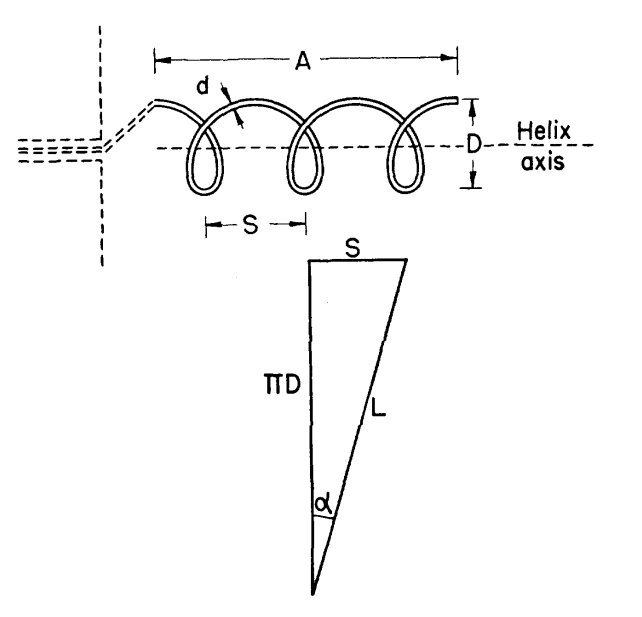
\includegraphics[width=0.40\textwidth]{parametros.png}
	\caption{Relación de dimensiones de la hélice}
	\label{fig:param}
\end{figure}

Normalmente, cuando se hable de dimensiones de la antena se hará en función de longitudes de onda (dimensiones eléctricas).

\subsection{Modos de transmisión y radiación de las hélices}
El campo electromagnético alrededor de la hélice puede ser tratado desde dos puntos de vista: como campo guiado y como campo radiado. Desde el primer punto de vista se asume que la onda electromagnética se propaga sin atenuación a lo largo de una hélice infinita, del mismo modo que lo haría por una linea de transmisión infinita. Esta propagación se puede describir por su \textit{modo de transmisión}. Por otro lado, el punto de vista del campo radiado se describe mediante el diagrama de radiación de la antena. Aunque son posibles una infinita variedad de diagramas, dos tipos son de particular interés dependiendo de la dirección del máximo de propagación: el modo de radiación normal y el modo de radiación axial.\\\\
El modo de transmisión de menor orden en un conductor helicoidal es el modo $T_{0}$. En él las regiones de carga positiva y negativa están separadas por varias vueltas. Es el modo de transmisión predominante cuando la longitud de una vuelta es mucho menor que la longitud de onda ($L<<\lambda$), común en inductores de baja frecuencia. Como las regiones adyacentes de carga están separadas por una distancia axial apreciable, aparece una componente axial de campo eléctrico. Esta componente interactúa con la onda viajera a lo largo de la hélice, dando lugar a campos radiados en la dirección normal. El caso más interesante asociado a este modo de transmisión se da cuando la longitud total de la antena es mucho menor que la longitud de onda ($nL<<\lambda$, siendo $n$ el número total de vueltas). En estas condiciones se puede asumir que las corrientes en la hélice tienen una magnitud y fase uniformes a lo largo de la estructura. De forma teórica, esta condición puede ser aproximada a una pequeña hélice cargada en su extremo en la que se produce una onda estacionaria. La impedancia de la antena se vuelve dependiente de la frecuencia y la eficiencia de radiación es pequeña. Esta combinación de antena pequeña con el modo de transmisión $T_{0}$ da lugar a antenas helicoidales con modo de radiación normal. La antena a diseñar requiere un modo de radiación axial, que no puede ser conseguido con este modo de transmisión.\\

\begin{figure}[h]
	\centering
	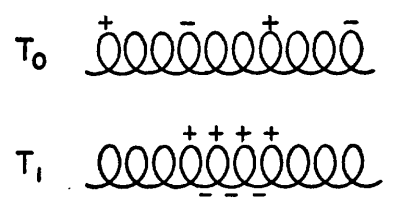
\includegraphics[width=0.3\textwidth]{modos.png}
	\caption{Distribución de las cargas para diferentes modos de transmisión}
	\label{fig:modes}
\end{figure}

El modo de transmisión de primer orden, designado como $T_{1}$, tiene las regiones de cargas positivas y negativas separadas aproximadamente por media vuelta de hélice, haciendo que queden diametralmente opuestas. Es el modo predominante cuando la longitud de una vuelta es del orden de una longitud de onda ($L\sim\lambda$). La radiación de este tipo de helices cuando $n>1$ tiene el máximo en la dirección de la hélice y está polarizada circularmente. Este tipo de radiación es el que se conoce como modo axial y es el que se quiere conseguir para la antena a diseñar. Una de las características más importantes de este modo de radiación es que se produce para un amplio rango de dimensiones de la hélice, haciendo que sea una de las antenas más fáciles de construir.\\\\
Los modos de radiación normal y axial son en realidad casos particulares de diagramas de radiación de antenas helicoidales. En el caso general, el máximo de radiación no estará ni en $\theta=0$ ni en $\theta=90º$, sino en un valor intermedio.

\subsection{Modo de radiación axial}
Las distribuciones de corriente de una antena helicoidal funcionando en modo axial pueden describirse como una onda viajera saliente más una onda viajera entrante de mucha menos magnitud. Cada onda está caracterizada por una región inicial de fuerte atenuación seguida de otra en la que la corriente es relativamente constante.\\

\begin{figure}[!h]
	\centering
	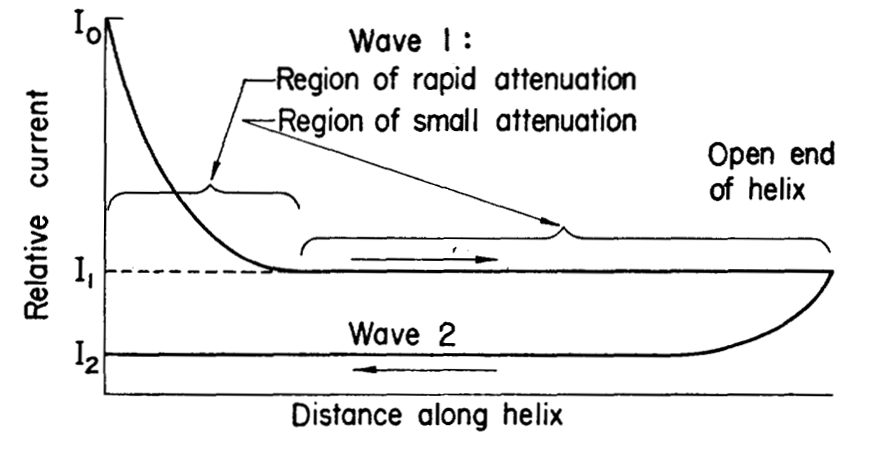
\includegraphics[width=0.6\textwidth]{ondas.png}
	\caption{Distribuciónes de corriente idealizadas}
	\label{fig:waves}
\end{figure}

La profunda atenuación de la onda reflejada (entrante) permite una distribución uniforme en la zona central en hélices largas. Ambas atenuaciones, tanto de la saliente como de la reflejada, explican la relativa estabilidad en impedancia de este tipo de antenas, ya que relativamente poca energía de la reflejada en el extremo llega a la entrada. Así, la SWR de corriente a la entrada es

\begin{equation*}
	SWR=\frac{I_{0}+I_{2}}{I_{0}-I_{2}}\approx 1
\end{equation*}

lo mismo que para una línea de transmisión cargada con su impedancia característica.\\\\
La velocidad de fase de la onda en la hélice es tal que hace que la componente del campo eléctrico en cada vuelta se sume aproximadamente en fase en la dirección del eje. La tendencia a que esto ocurra es lo suficientemente fuerte para que la velocidad de fase se ajuste por si misma para producir este resultado. Este ajuste natural es el que hace que el modo axial tenga su persistencia característica.\\\\
La velocidad de fase es aproximadamente igual a la velocidad de la luz en el vacío cuando la frecuencia es muy baja para el modo de radiación axial. Si se aumenta la frecuencia, aparece un rango frecuencial en el que la velocidad de fase es menor. En este rango es en el que radia en  dirección axial.

\subsection{Factor de agrupación}
Como aproximación, se asume que en modo axial se tiene una única onda viajera saliente en el conductor. El diagrama de la hélice es calculado como una agrupación de vueltas individuales, todas con el mismo diagrama de radiación. Cuando la antena es lo suficientemente larga ($nS$ grande), el factor de agrupación se vuelve dominante y determina casi por completo la forma del diagrama. Así, aunque las componentes de polarización vertical y horizontal de cada vuelta son muy diferentes, las componentes de la hélice completa son prácticamente iguales.\\\\
Para calcular el factor de agrupación, la hélice de $n$ vueltas se remplaza por $n$ fuentes puntuales isotrópicas.

\begin{equation}
	FA(\psi)=\frac{\sin\frac{n\psi}{2}}{\sin\frac{\psi}{2}}
\end{equation} 

La fase con la que la onda radiada por la \textit{fuente 1} llega a un punto arbitrario $P$ está adelantada a la fase de la onda proveniente de la \textit{fuente 2} por $2\pi S_{\lambda}\cos\theta$, pero retardada por $2\pi L_{\lambda}/p$, donde $p$ es el factor de velocidad de fase ($p=v/c$). Este retardo es proporcional al tiempo requerido para que la onda viaje a lo largo de una vuelta, de la fuente 2 a la 1. El valor del ángulo eléctrico $\psi$ es la diferencia.

\begin{equation}
	\psi=2\pi(S_{\lambda}\cos\theta-\frac{L_{\lambda}}{p})
\end{equation} 

Las ondas llegan a $P$ en fase cuando $\psi=-2\pi m$ y $\theta=0$, donde $m$ es un entero $(0,1,2,...)$. Se puede extraer la siguiente condición:

\begin{equation}
	\frac{L_{\lambda}}{p}=m+S_{\lambda}
\end{equation} 

La expresión (3) se relaciona de forma directa con los modos de transmisión comentados en la sección 2.1, ya que es una relación aproximada para que por el conductor se propaguen los diferentes modos $T_{m}$. Así, para el modo $T_{1}$, que es el que produce radiación axial, tenemos:

\begin{equation}
	\frac{L_{\lambda}}{p}=1+S_{\lambda}\longrightarrow\frac{L}{p}=\lambda+S
\end{equation} 

Introduciendo la relación $L²=S²+(\pi D)²$, se obtiene una interrelación entre los parámetros de espaciado ($S$) y diámetro ($D$) para que la antena radie en modo axial.\\

\begin{figure}[!h]
	\centering
	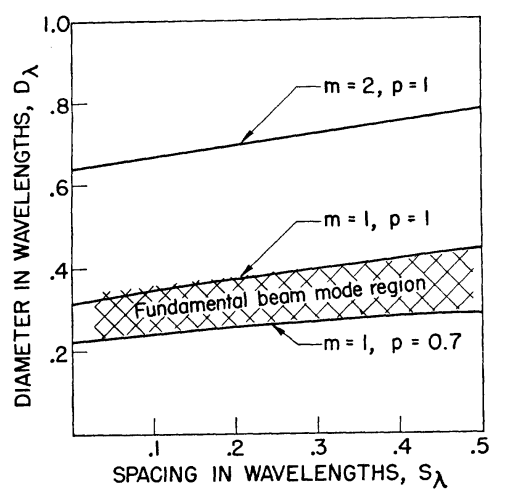
\includegraphics[width=0.4\textwidth]{diametro_espaciado.png}
	\caption{Diámetro vs espaciado}
	\label{fig:diam_vs_spacing}
\end{figure}

El factor de velocidad de fase debe estar entre $p=1$ y $p=0,7$ 
\newpage

\section{Diseño de la antena}
Conocidos los fundamentos teóricos se procede a diseñar y simular la antena. Los parámetros se obtienen a partir de las condiciones de diseño del modo axial descritas en la siguiente tabla.

\begin{table}[!h]
\centering
\begin{tabular}{lc}
	\hline 
	\textit{Parámetro} & \textit{Valor} \\ 
	\hline 
	\hline
	Circunferencia ($\pi D$) & $3\lambda/4 < C < 4\lambda/3$  \\ 
	\hline 
	$S$ & $0.19\lambda < p < 0.25\lambda$ \\ 
	\hline 
	$ \alpha $ & $ 11 \lambda < \alpha  < 15 \lambda $ \\ 
	\hline 
	$n$ & $3 < n < 15$  \\ 
	\hline 
	Diámetro del plano de tierra & $D_{GND} > 0,8\lambda$ \\ 
	\hline 
	Diámetro del conductor ($d$)	& $ 0.001\lambda < d < 0.01 \lambda$   \\ 
	\hline 
	Impedancia de entrada & Sensible a la alimentación. Entre 140 y 250 $\Omega$  \\ 
	\hline 
\end{tabular}
\caption{Condiciones de diseño para antena helicoidal en modo axial}
\label{table:condiciones_diseno}
\end{table} 

El diseño óptimo se tiene para $C \simeq \lambda_0$ y $\alpha \simeq 13°$, siendo $\lambda_0$ la longitud de onda en el vacío. Fijando estos parámetros se obtienen $S$ y $L$:\\
\begin{equation}
S = C \tan{\alpha} = \lambda_0 \tan(13°) = 0.231 \lambda_0 
\end{equation}
\begin{equation}
L=\sqrt{S^2 + C^2} = \lambda_0 \sqrt{(0.231)^2 + (1)^2} = 1.0263 \lambda_0
\end{equation}

Con estas condiciones de diseño se van a simular distintas antenas variando parámetros como el plano de tierra utilizado. Así se pretenden analizar variaciones de ganancia, diagrama de radiación, NLPS, polarización, etc. Para la simulación se ha elegido \textit{4nec2}, ya que es un software gratuito y para antenas de tipo hilo ofrece buenos resultados. Este software calcula mediante el método de momentos la respuesta electromagnética de antenas y estructuras metálicas. El programa viene con un generador de geometrías que se puede utilizar para generar un archivo \textit{.nec} con los segmentos del reflector o la hélice.

\subsection{Antena con plano de tierra infinito}
Se empieza simulando una hélice unifilar de 7 vueltas con plano de tierra infinito y frecuencia central de 435 MHz ($\lambda_0 = 68.965cm$). El hilo utilizado es de 2.5mm de diámetro. El espaciado $S$ según (5) es de aproximadamente 16cm; y el diámetro $D$, con $C=\lambda_0$, es de 22cm.\\\\
Obtenidos los valores, se crea el archivo \textit{.nec} indicando la geometría, las excitaciones y la frecuencia de trabajo.\\

\begin{lstlisting}[caption={Archivo .nec con la confifuración de la estructura},captionpos=b]
	CM Helice 435 MHz (7 vueltas), plano de tierra perfecto inifinito
	CM La helice empieza 5mm sobre el plano de tierra
	CM Diametro de la helice 22cm, espaciado de 16cm
	CM Hilo de 2.5 mm entre tierra y helice
	CM La excitacion se aplica sobre este hilo
	CE
	CM	Tag	Seg	S		A		D/2		D/2		D/2		D/2		d/2
	GH	1	120	0.16	1.115	0.11	0.11	0.11	0.11	0.00125
	CM Subimos la helice 5mm
	GM	0	0	0	0	0	0	0	0.005	0
	CM Anadimos tramo de 5mm (coaxial SMA)
	GW	150	1	.11	0	0	0.11	0	0.005	0.00125
	GE	1
	CM Plano de tierra
	GN	1
	EK
	CM Fuente de voltaje 1V
	EX	0	150	1	0	1.	0	0
	FR	0	0	0	0	435	0
	EN
\end{lstlisting}

Este archivo se carga en \textit{4nec2} y se calcula la radiación en campo lejano para un barrido de frecuencias entre 400 y 500 MHz.\\

\begin{figure}[!h]
	\centering
	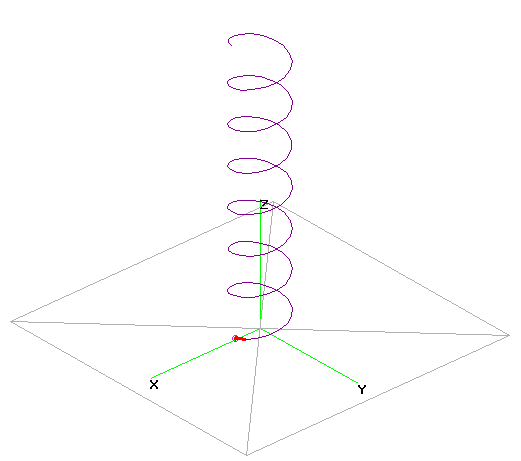
\includegraphics[width=0.42\textwidth]{helix_1.png}
	\caption{Estructura en \textit{4nec2}}
	\label{fig:estructura}
\end{figure}

\subsubsection*{Ganancia y NLPS}

En la Figura 6 se muestran los diagramas de radiación a diferentes frecuencias. A 400 MHz se tiene una ganancia máxima de 9,92 dBi. Conforme aumenta la frecuencia el ancho de haz se va estrechando y la ganancia aumenta hasta 11.8 dBi a 500 MHz. Este incremento ocurre en todo el rango analizado.\\\\
Por otro lado, la relación NLPS no responde de una manera uniforme a la frecuencia. Así, a 400 MHz no aparece ningún lóbulo secundario y conforme aumenta la frecuencia empiezan a aparecer. Llega un momento en que el aumento de ganancia de los lóbulos secundarios disminuye en relación al del principal y el NLPS mejora: a 450 MHz el NLPS es de 7 dB, mientras que a 500 MHz es de 9,64 dB.\\

\begin{figure}[H]
	\centering
	\begin{subfigure}{.48\textwidth}
		\centering
		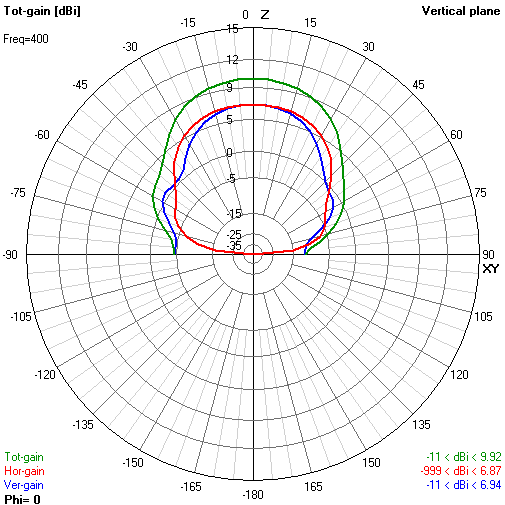
\includegraphics[width=.75\linewidth]{helix_1_400.png}
		\caption{400 MHz}
	\end{subfigure}%
	\begin{subfigure}{.48\textwidth}
		\centering
		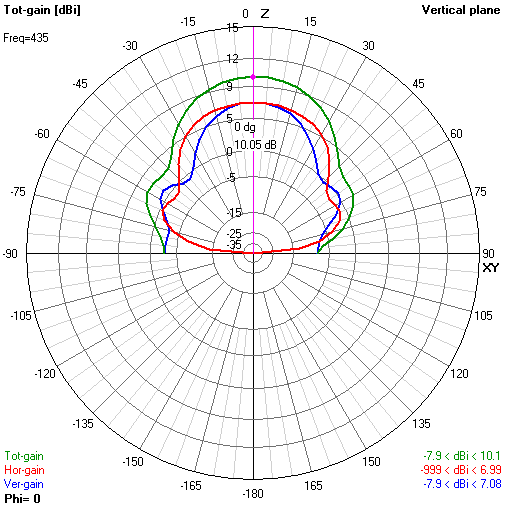
\includegraphics[width=.75\linewidth]{helix_1_435.png}
		\caption{435 MHz}
	\end{subfigure}
	\begin{subfigure}{.48\textwidth}
		\centering
		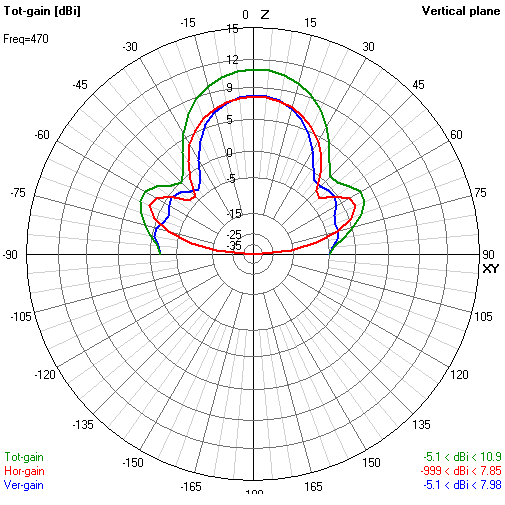
\includegraphics[width=.75\linewidth]{helix_1_470.png}
		\caption{470 MHz}
	\end{subfigure}
	\begin{subfigure}{.48\textwidth}
		\centering
		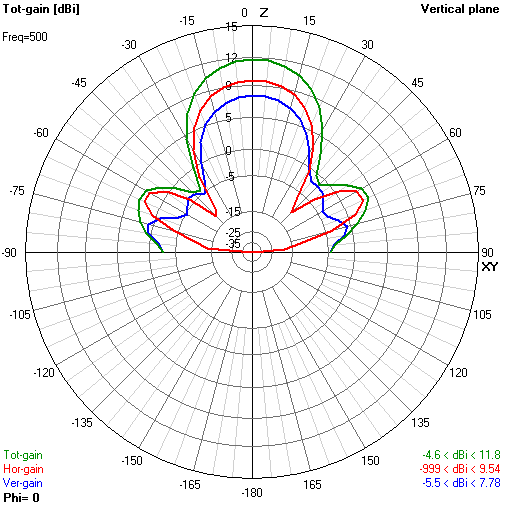
\includegraphics[width=.75\linewidth]{helix_1_500.png}
		\caption{500 MHz}
	\end{subfigure}
	\caption{Diagramas de radiación para distintas frecuencias con plano de tierra infinito}
\end{figure}

\subsubsection*{Polarización}

La información acerca de la polarización no se puede obtener de forma explícita en \textit{4nec2}. Para extraerla, hay que exportar el archivo de texto donde se almacena la magnitud de los campos radiados en $\phi$ y en $\theta$. Con este archivo se calcula en \textit{Matlab} la relación axial dividiendo el valor de las componentes del campo en el semieje mayor entre las del menor para cada frecuencia. La relación axial es 0 dB cuando se tiene polarización circular, y cualquier otro valor para el caso elíptico ($\infty$ para polarización lineal). El sentido de giro predominante puede conocerse comparando los valores de RHCP y LHCP. En la Figura 7 se muestran estos valores en la dirección del máximo para un barrido de frecuencias entre 400 y 500 MHz. La polarización es circular dextrógira en casi todo el rango analizado.\\

\begin{figure}[!h]
	\centering
	\begin{subfigure}{.45\textwidth}
		\centering
		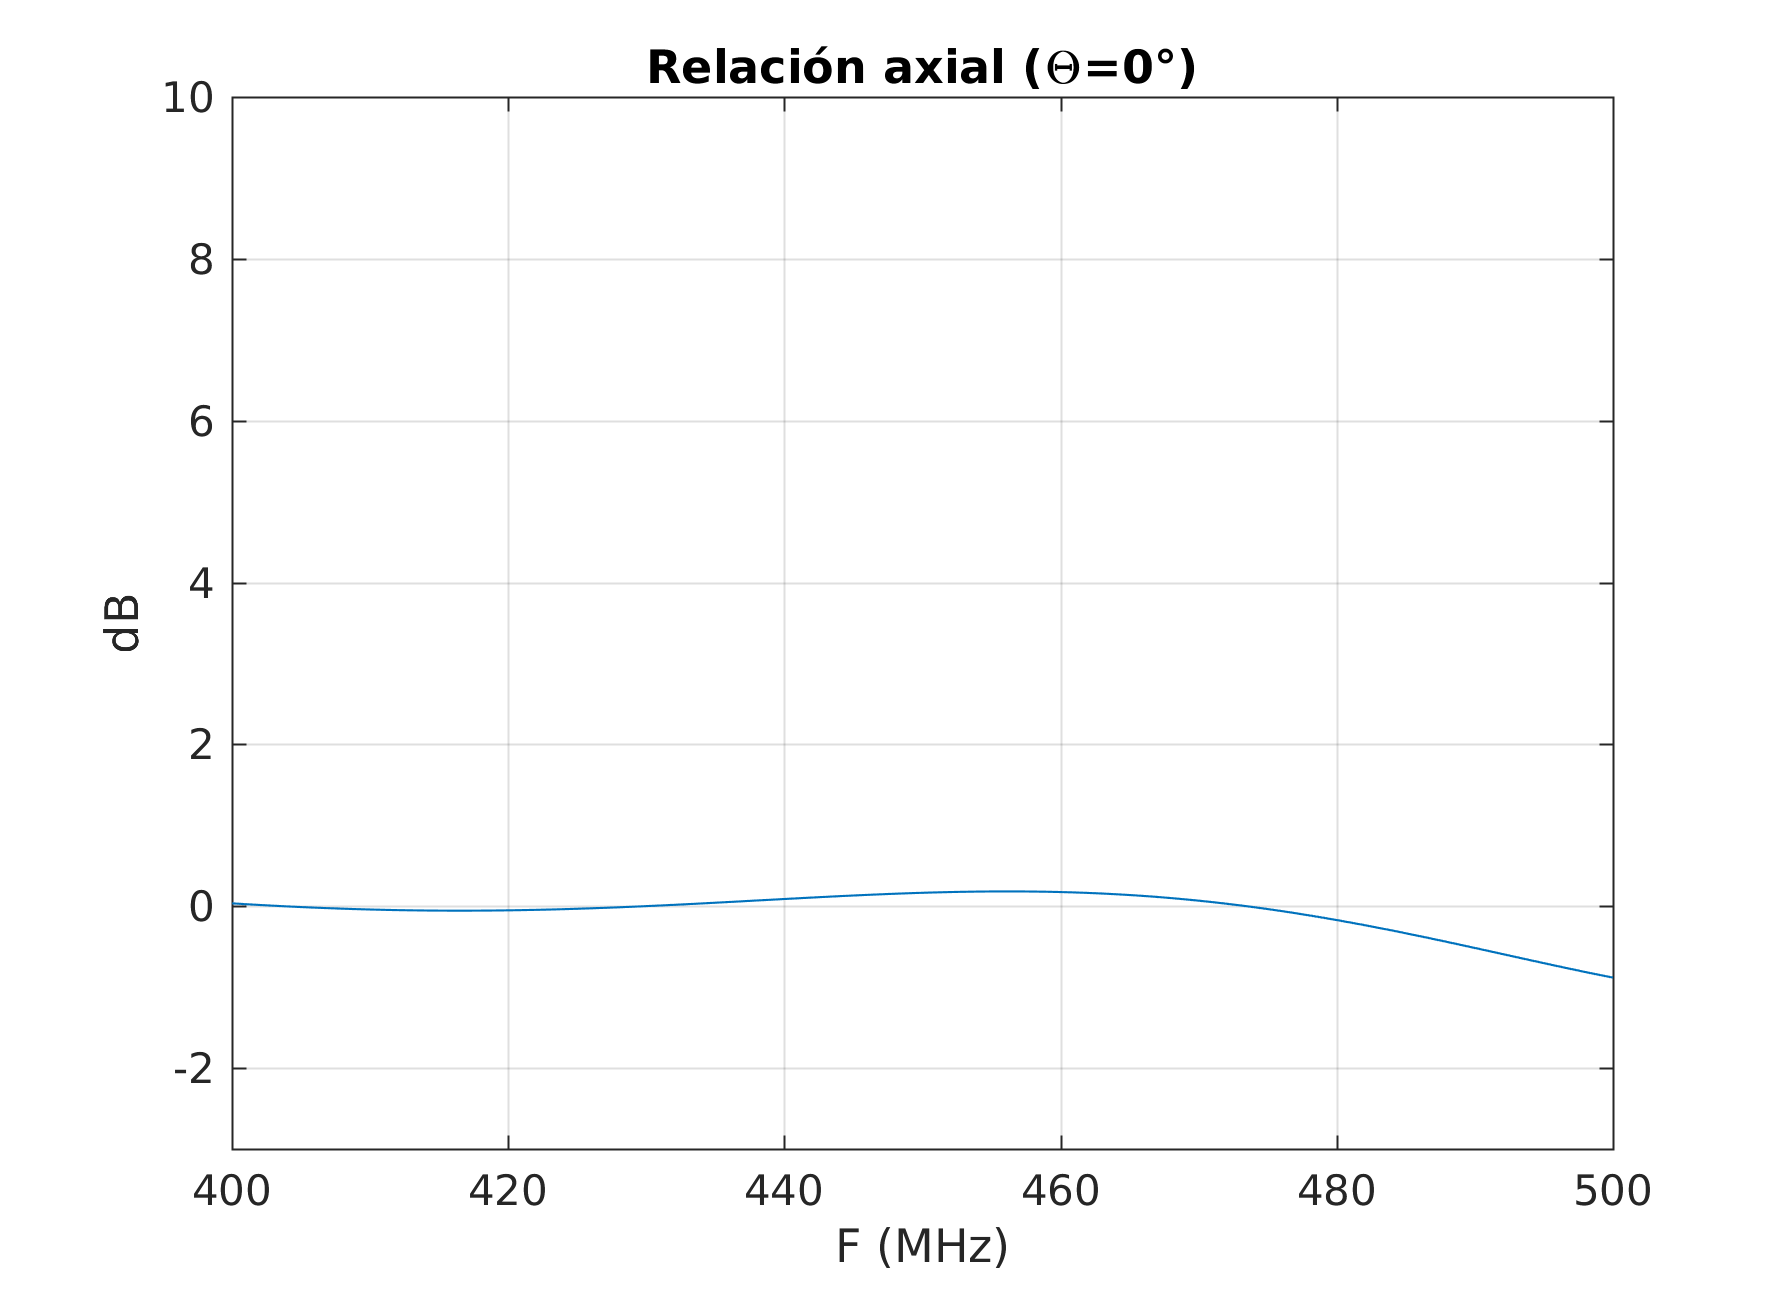
\includegraphics[width=1.1\linewidth]{helix_1_THETA0_AR.png}
		\caption{Relación axial}
	\end{subfigure}%
	\begin{subfigure}{.45\textwidth}
		\centering
		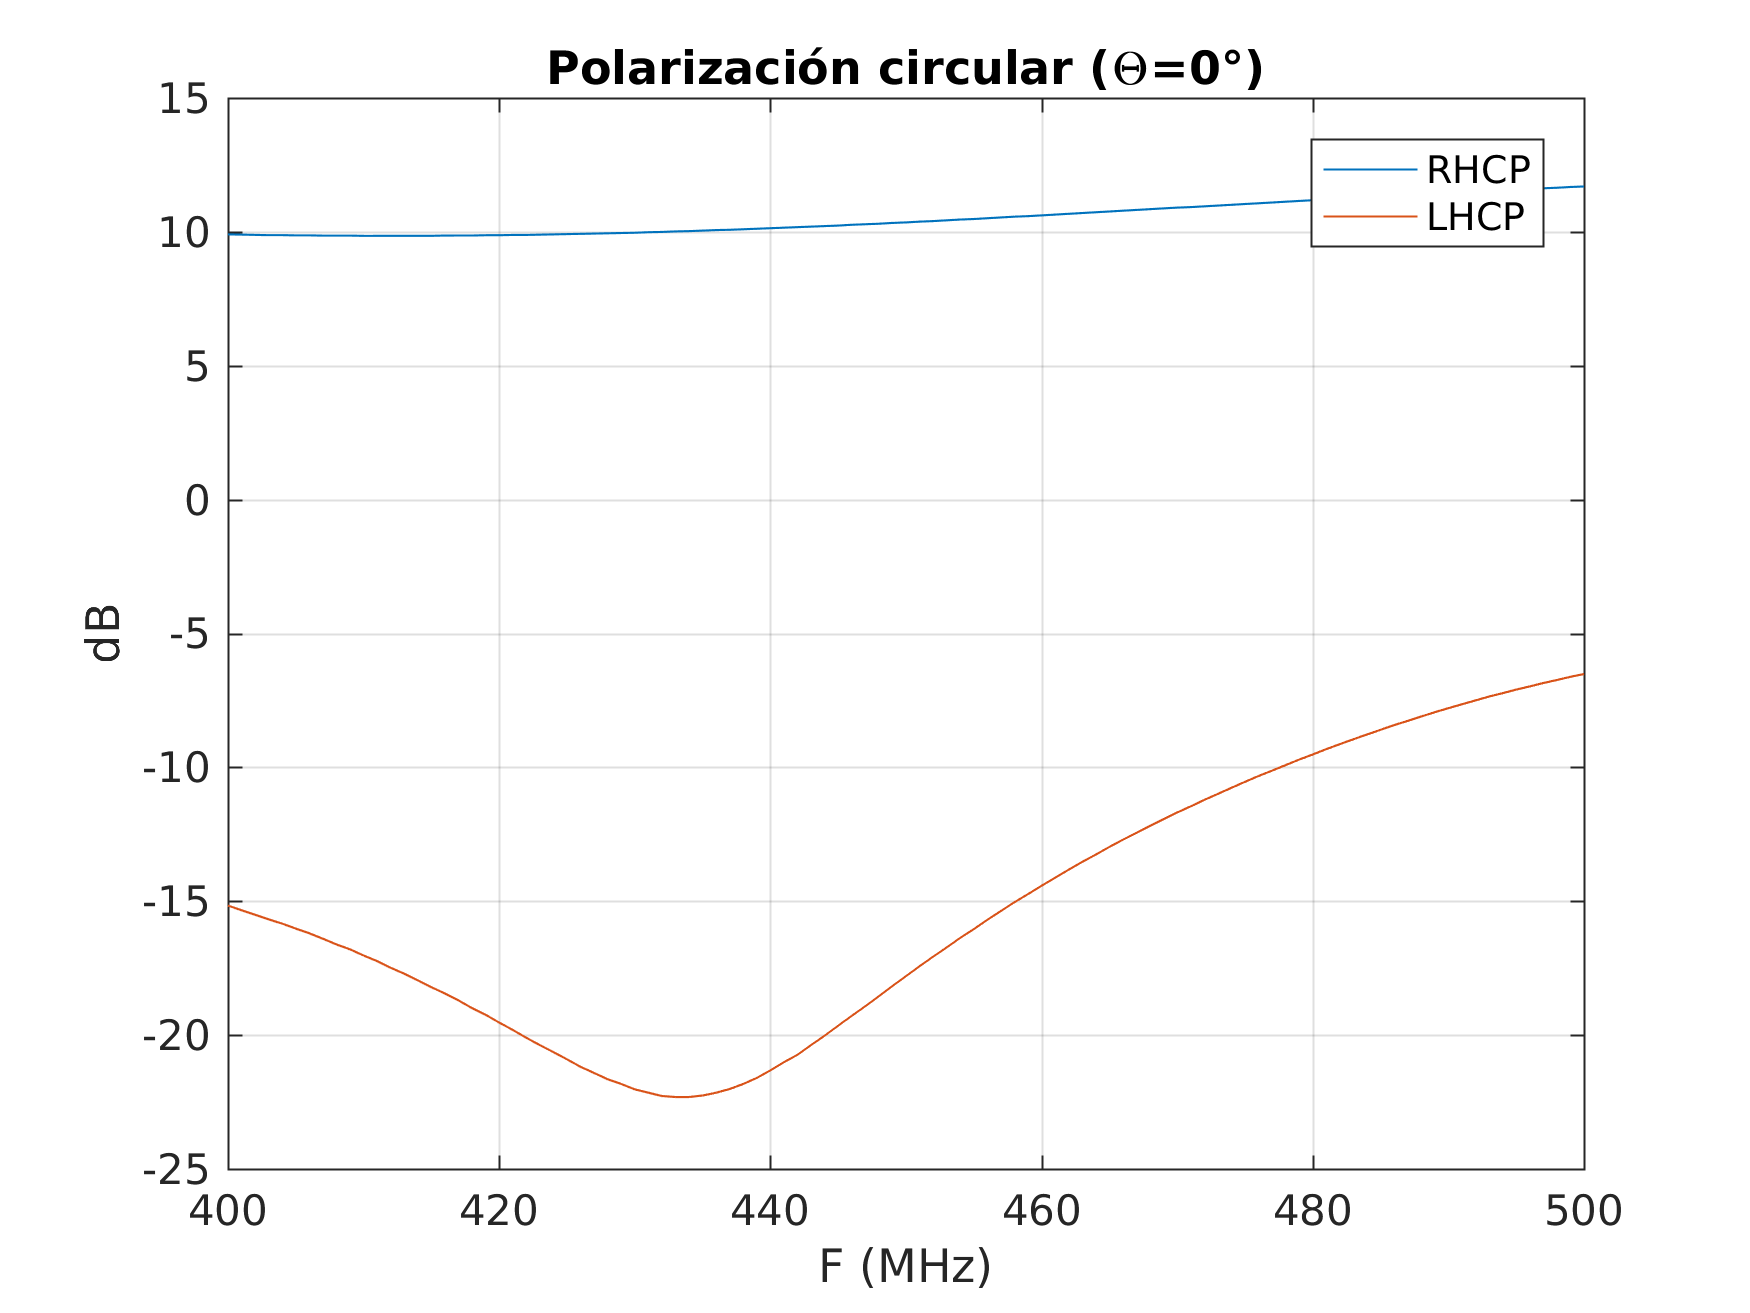
\includegraphics[width=1.1\linewidth]{helix_1_THETA0_CP.png}
		\caption{RHCP/LHCP}
	\end{subfigure}
	\caption{Polarización en la dirección del máximo ($\theta=0$)}
\end{figure}

Se puede concluir que la antena presenta un alto ancho de banda desde el punto de vista de la polarización. De momento sólo se ha obtenido información en la dirección del máximo. En la Figura 8 se muestran los mismos datos de polarización para la frecuencia de diseño, esta vez barriendo $\theta$.\\\\
La polarización no es uniforme en este caso. Considerando el criterio de relación axial menor que 3 dB, el ancho de haz con polarización circular es de unos 160º. Este ancho es muy grande, más aún teniendo en cuenta que la antena está diseñada para trabajar con ángulos muy cerrados, por lo que si tiene uniformidad en la práctica. La predominancia de la polarización dextrógira también es uniforme en la zona de trabajo, aunque es interesante ver que existe una componente levógira fuera del eje de la antena.\\

\begin{figure}[!h]
	\centering
	\begin{subfigure}{.45\textwidth}
		\centering
		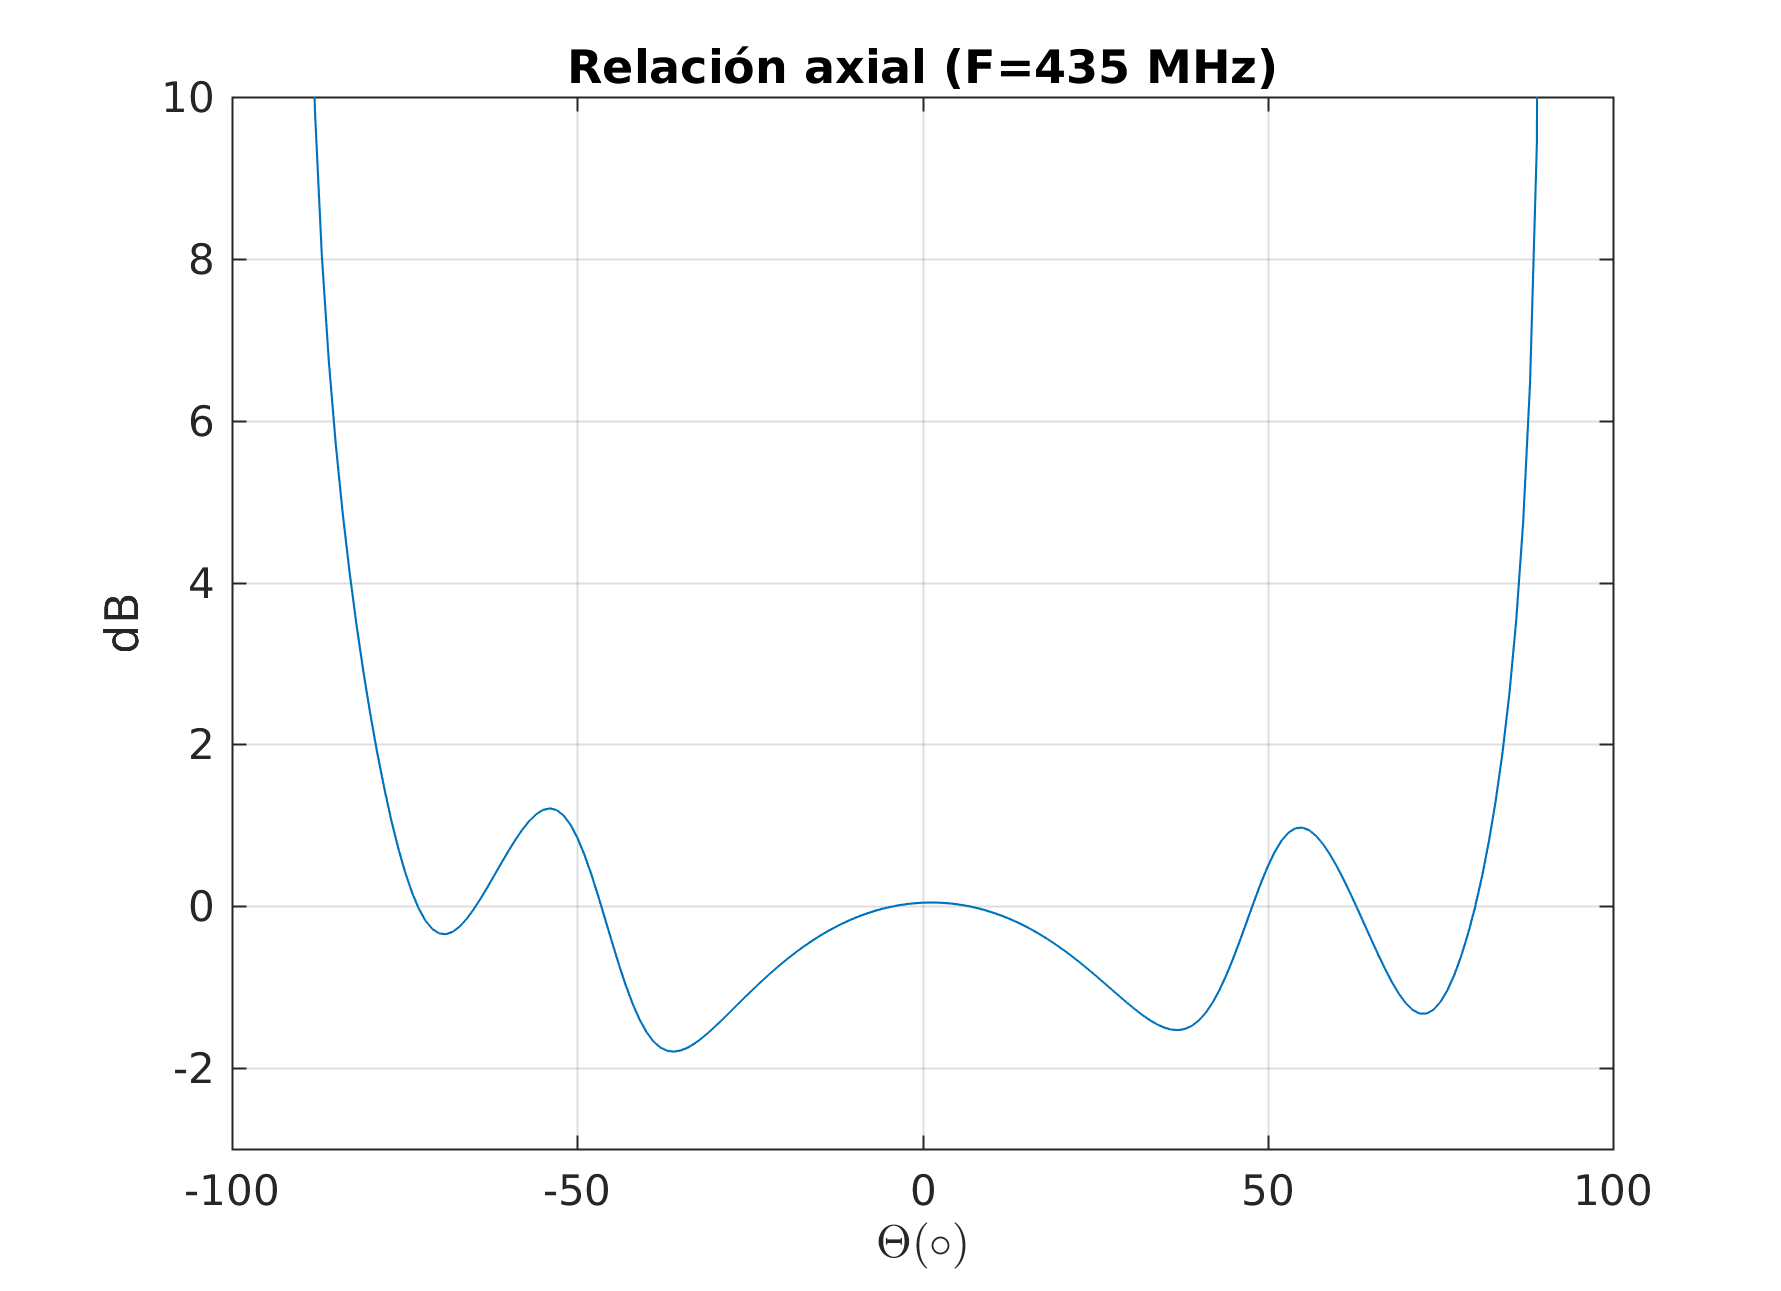
\includegraphics[width=1.1\linewidth]{helix_1_F435_AR.png}
		\caption{Relación axial}
	\end{subfigure}%
	\begin{subfigure}{.45\textwidth}
		\centering
		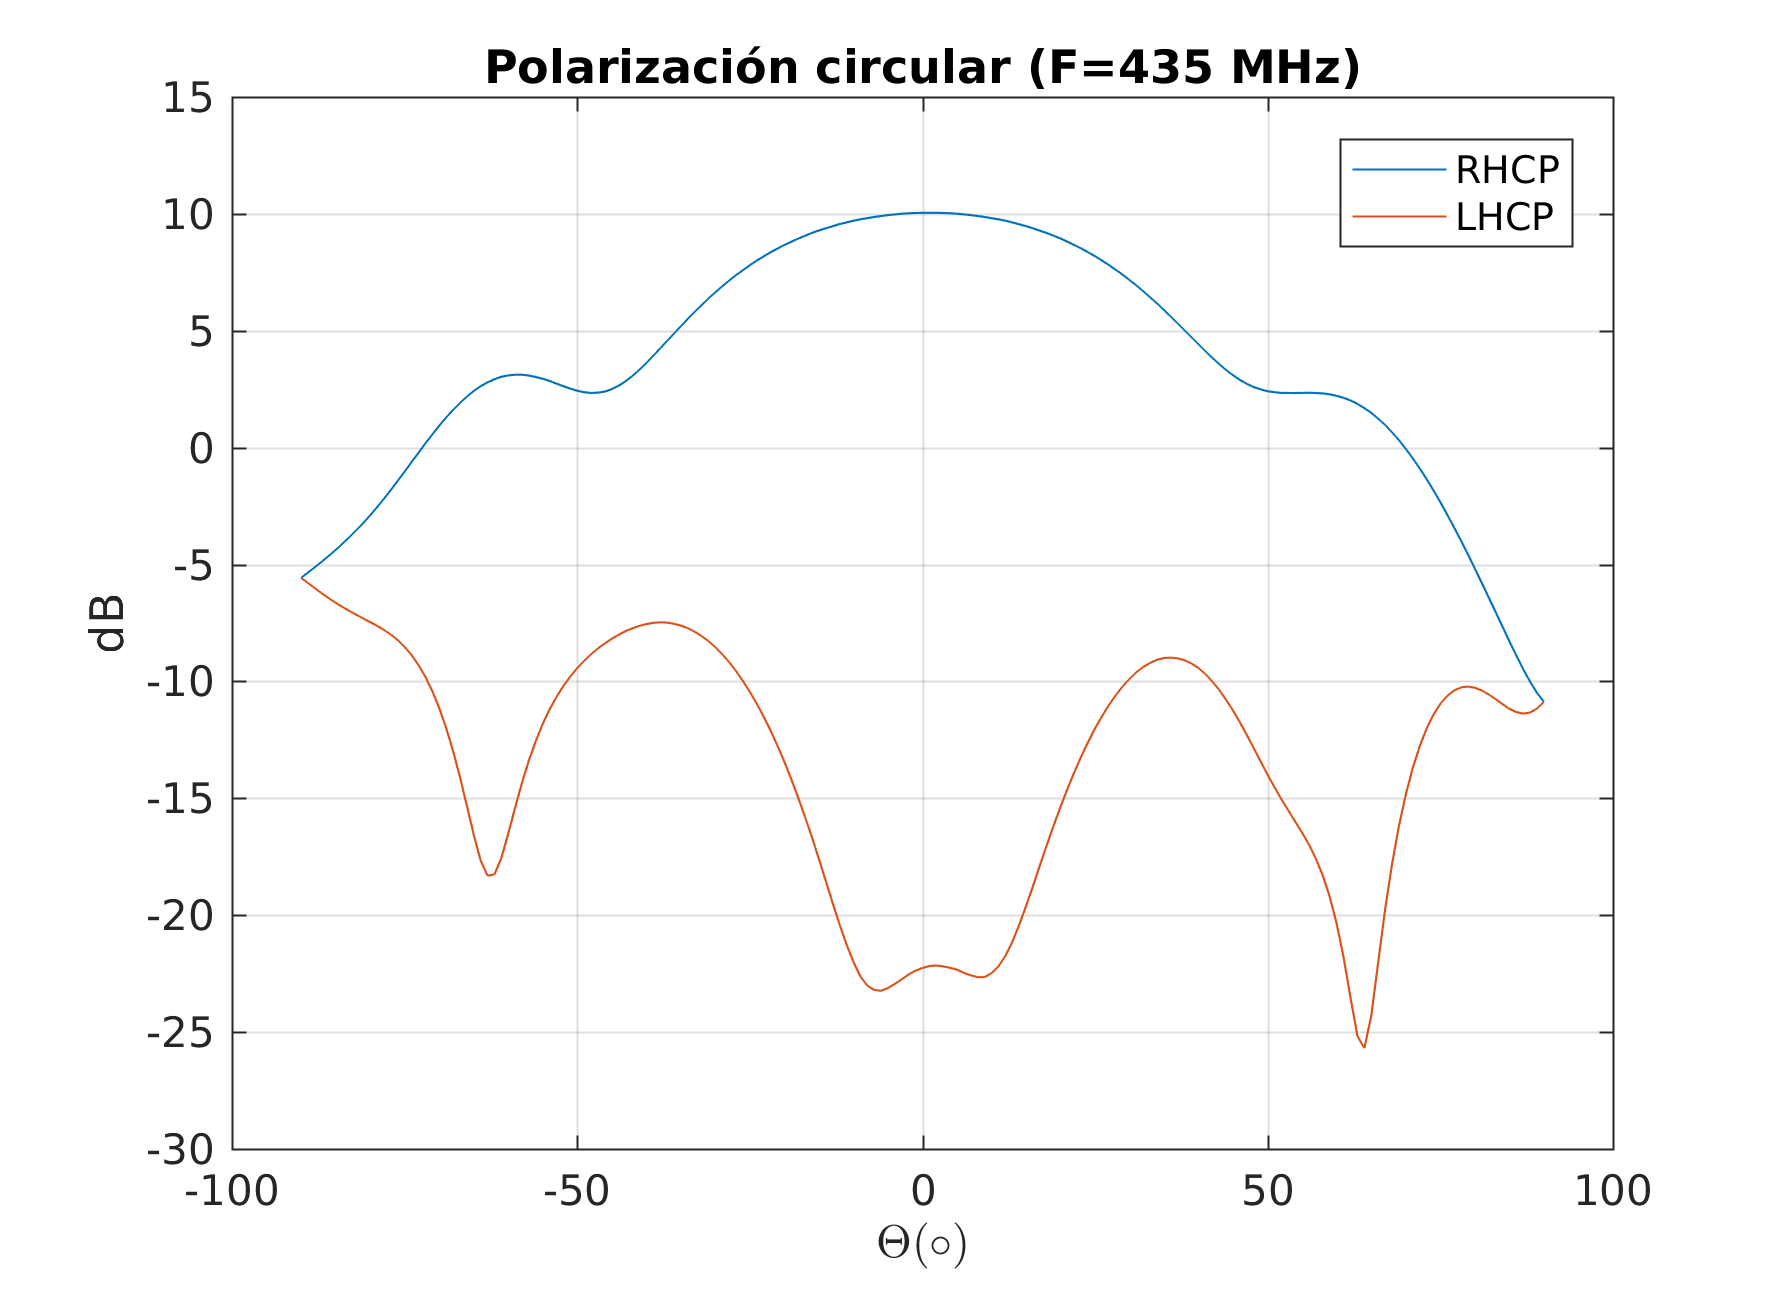
\includegraphics[width=1.1\linewidth]{helix_1_F435_CP.png}
		\caption{RHCP/LHCP}
	\end{subfigure}
	\caption{Polarización a 435 MHz (barrido en $\theta$)}
\end{figure}

\subsubsection*{Impedancia de entrada}

La impedancia de entrada se mantiene más o menos constante en un amplio rango de frecuencias. Los valores resistivos están dentro de lo esperado, sin embargo presenta una componente reactiva elevada. Será necesaria una red de adaptación que baje la impedancia a 50$\Omega$ manteniendo el mayor ancho de banda posible.\\

\begin{figure}[!h]
	\centering
	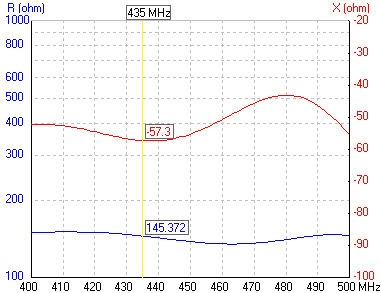
\includegraphics[width=0.5\textwidth]{zin.png}
	\caption{Impedancia de entrada}
\end{figure}

\subsection{Variación del número de vueltas}
Se ha visto en los fundamentos teóricos que existe un óptimo de $L$ y de $S$ para una determinada frecuencia central. La geometría se puede variar en dos aspectos: el grosor del hilo, que ya se ha comentado en la teoría que no produce grandes cambios; y el número de vueltas, que se estudiará a continuación.

\subsubsection*{Antena de 4 vueltas}
Se comienza simulando una antena de 4 vueltas con el resto de parámetros idénticos al diseño inicial.\\

\begin{figure}[H]
	\centering
	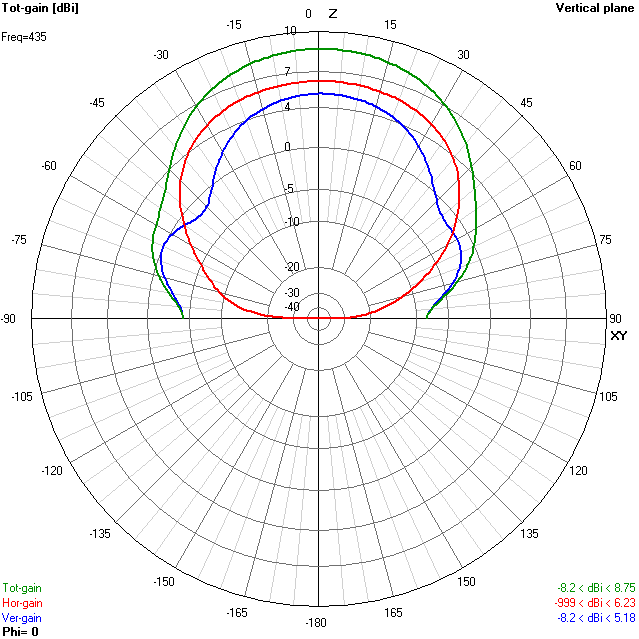
\includegraphics[width=0.5\textwidth]{helix_4_435_gain.png}
	\caption{Diagrama de radiación con 4 vueltas a 435 MHZ}
\end{figure}

El diagrama de radiación es similar al de la antena de 7 vueltas y se comporta de forma parecida con la frecuencia. La ganancia empeora (de 10,1 dBi a 8,75 dbi a 435 MHz) aunque se mantiene constante en todo el rango. El NLPS también empeora (de 9,64 dB a 7,81 dB a 500 MHz).\\\\
La resistencia también es constante y un poco más alta. La reactancia varía más con la frecuencia.\\

\begin{figure}[H]
	\centering
	\begin{subfigure}{.45\textwidth}
		\centering
		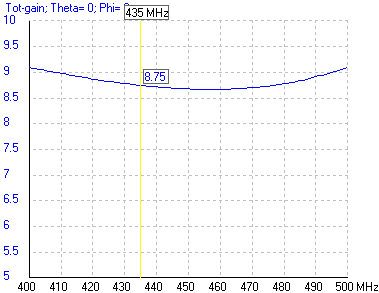
\includegraphics[width=0.9\linewidth]{helix_4_sweep_gain.png}
		\caption{Ganancia}
	\end{subfigure}%
	\begin{subfigure}{.45\textwidth}
		\centering
		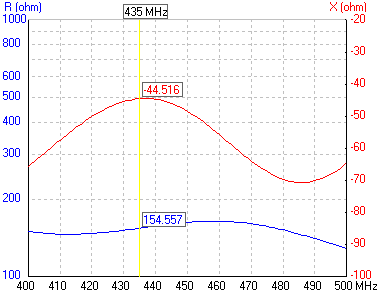
\includegraphics[width=0.9\linewidth]{helix_4_sweep_zin.png}
		\caption{Impedancia de entrada}
	\end{subfigure}
	\caption{Barridos en frecuencia con 4 vueltas}
\end{figure}

La polarización se mantiene circular en todo el ancho de banda como demuestra la relación axial de la Figura 12.\\

\begin{figure}[H]
	\centering
	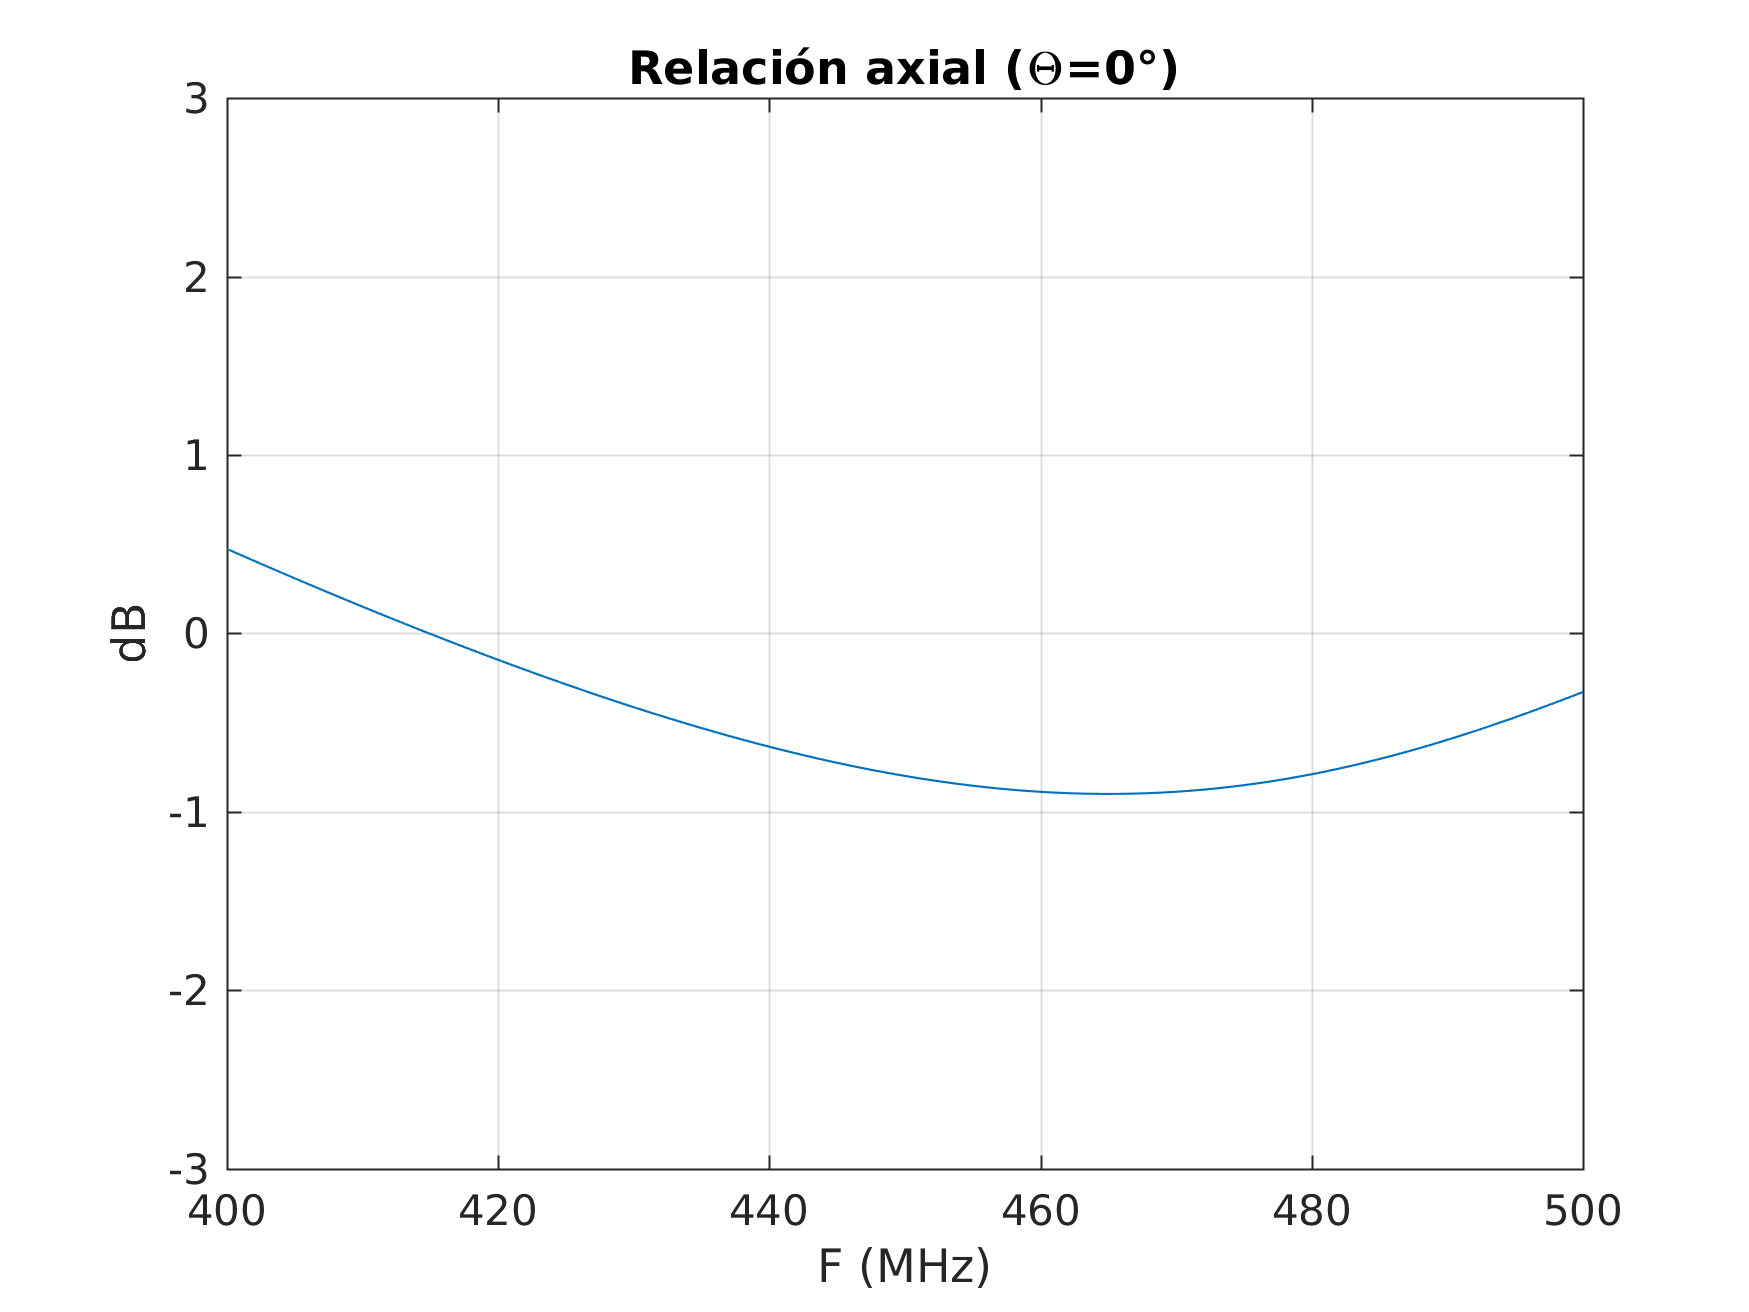
\includegraphics[width=0.5\textwidth]{helix_4_sweep_AR.png}
	\caption{Relación axial antena de 4 vueltas}
\end{figure}


\subsubsection*{Antena de 10 vueltas}
Reduciendo el número de vueltas las prestaciones empeoran. Cabe pensar que incrementándolas mejoren, a costa de una antena de mayor tamaño. La antena se tiene que montar sobre el soporte de un tracker, por lo que no puede ser demasiado grande.\\

\begin{figure}[H]
	\centering
	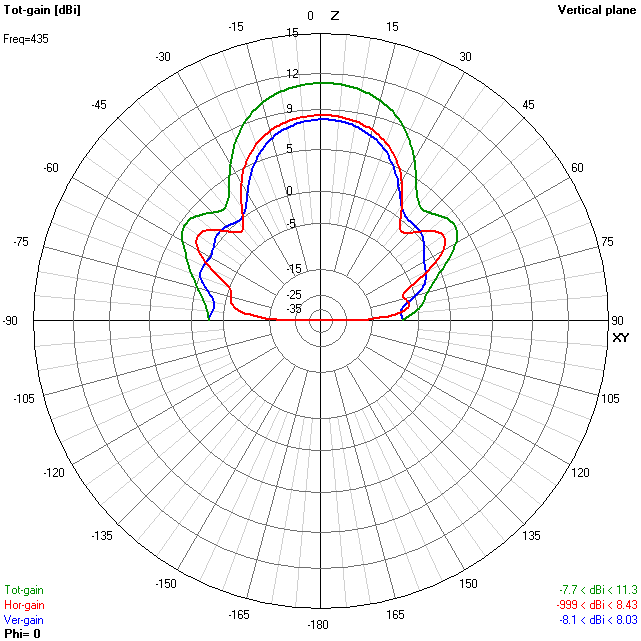
\includegraphics[width=0.5\textwidth]{helix_10_435_gain.png}
	\caption{Diagrama de radiación con 10 vueltas a 435 MHZ}
\end{figure}

La ganancia aumenta hasta 11,3 dBi a 435 MHz. Sin embargo, aparecen lóbulos secundarios que hacen que el NLPS empeore. A la frecuencia de diseño se tiene una relación de 6,5 dB.\\\\
En cuanto al resto de parámetros, se sigue teniendo banda ancha.\\

\begin{figure}[H]
	\centering
	\begin{subfigure}{.45\textwidth}
		\centering
		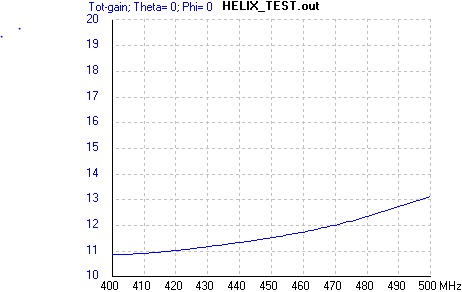
\includegraphics[width=1.1\linewidth]{helix_10_sweep_gain.png}
		\caption{Ganancia}
	\end{subfigure}%
	\begin{subfigure}{.45\textwidth}
		\centering
		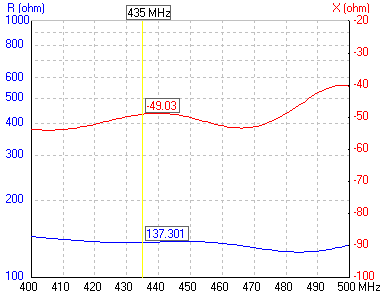
\includegraphics[width=0.9\linewidth]{helix_10_sweep_zin.png}
		\caption{Impedancia de entrada}
	\end{subfigure}
	\caption{Barridos en frecuencia con 10 vueltas}
\end{figure}


\begin{figure}[H]
	\centering
	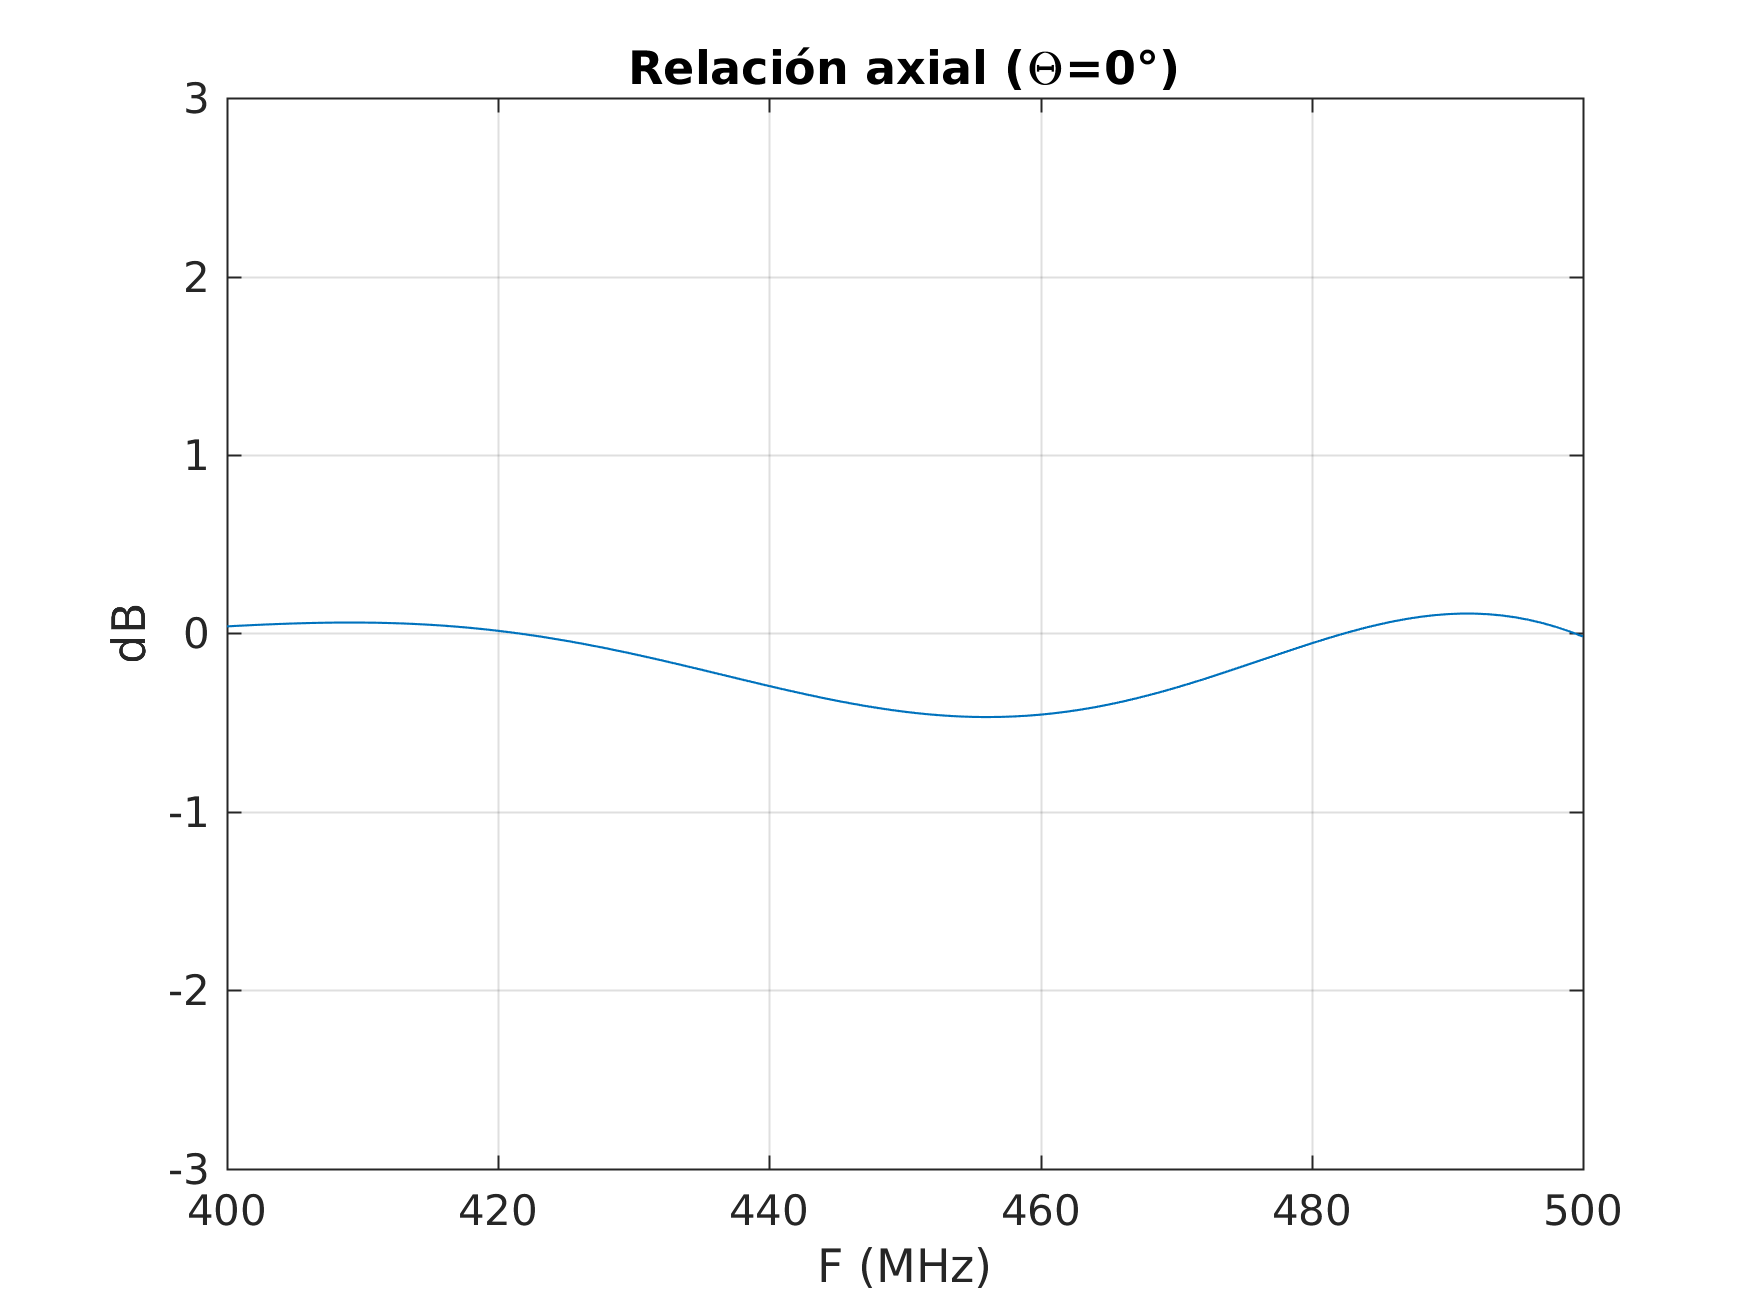
\includegraphics[width=0.5\textwidth]{helix_10_sweep_AR.png}
	\caption{Relación axial antena de 10 vueltas}
\end{figure}

\subsubsection*{Conclusiones}
Las prestaciones mejoran mucho con el número de vueltas, pero una antena de 10 vueltas tiene demasiado tamaño para ser montada en un tracker. Con una separación entre vueltas de 16 cm la longitud total es de 1,6 m. Por ello, se opta por el diseño original de 7 vueltas.\\\\
Hay que recordar que este diseño no es real, puesto que tiene un plano de tierra infinito. en la siguiente sección se visualizará el efecto de reducir el plano a dimensiones finitas.\\\\
Para concluir, en el Cuadro 2 se hace un resumen de las prestaciones de la antena de 7 vueltas a la frecuencia de diseño.\\

\begin{table}[!h]
	\centering
\begin{tabular}{lc}
	\hline 
	Frecuencia [MHz] & $435$ \\ 
	\hline 
	Ganancia [dBi] & $10.1$ \\ 
	\hline 
	NLPS [dB] & $7.65$ \\ 
	\hline 
	Relación axial [dB] & $0.043$ \\ 
	\hline 
	$Z_{in}$ [$\Omega$] & $145.4 - j57.3$ \\ 
	\hline 
\end{tabular} 
\caption{Antena con plano de tierra infinito}
\end{table} 
\newpage

\subsection{Antena con plano de tierra finito}
Sólo se va a ver el efecto del plano a la frecuencia de diseño en la antena de 7 vueltas. Parte de la radiación saldrá hacia atrás debido a la difracción en los bordes del plano. No se estudiará el efecto del plano sobre el ancho de banda, que se considerará invariante en el rango de frecuencias estudiado hasta este punto. Los siguientes resultados se obtienen con un plano de tierra de diámetro $0,8\lambda$. Este se genera con la herramienta Geometry Builder de \textit{4nec2}. El archivo que se crea se añade al \textit{.nec} de la antena.

\begin{figure}[H]
	\centering
	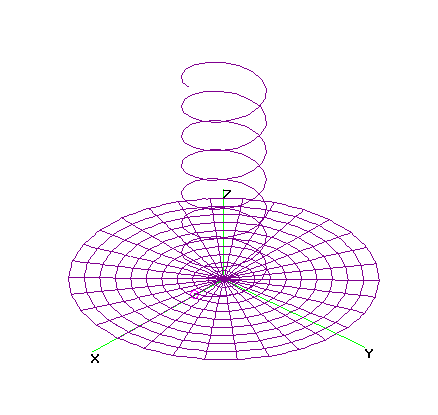
\includegraphics[width=0.45\textwidth]{antena_planotierra.png}
	\caption{Estructura con plano de tierra en \textit{4nec2}}
\end{figure}

Con un simple vistazo al diagrama de radiación puede verse que el efecto del plano de tierra tiene una gran influencia en los parámetros de la antena. El haz se estrecha y aparecen lóbulos en la dirección backfire. La directividad aumenta de 10,1 a 12,9 dBi. El NLPS mejora a 14 dB (antes 6,5 dB). En términos generales, la radiación se concentra más en el eje de la antena.\\

\begin{figure}[H]
	\centering
	\begin{subfigure}{.45\textwidth}
		\centering
		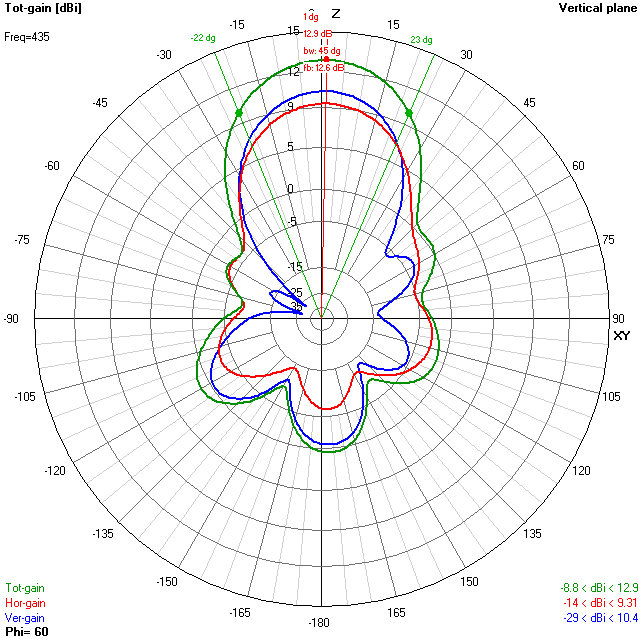
\includegraphics[width=0.9\linewidth]{gp_rad_435.png}
		\caption{Plano de tierra finito}
	\end{subfigure}%
	\begin{subfigure}{.45\textwidth}
		\centering
		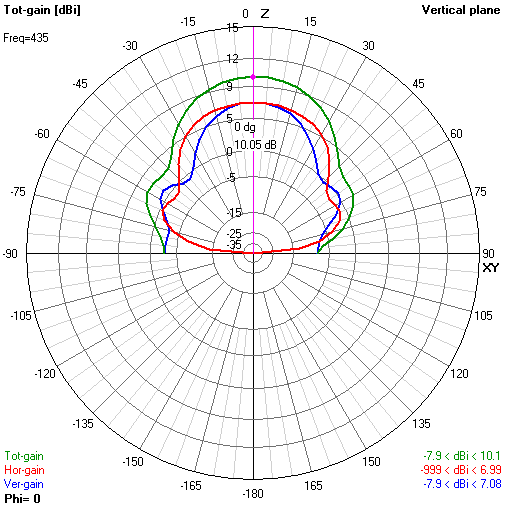
\includegraphics[width=0.9\linewidth]{helix_1_435.png}
		\caption{Plano de tierra infinito}
	\end{subfigure}
	\caption{Comparativa entre diagramas de radiación de antenas de 7 vueltas}
\end{figure}

La polarización se mantiene circular en el haz principal pero se vuelve inestable fuera de él.\\

\begin{figure}[H]
	\centering
	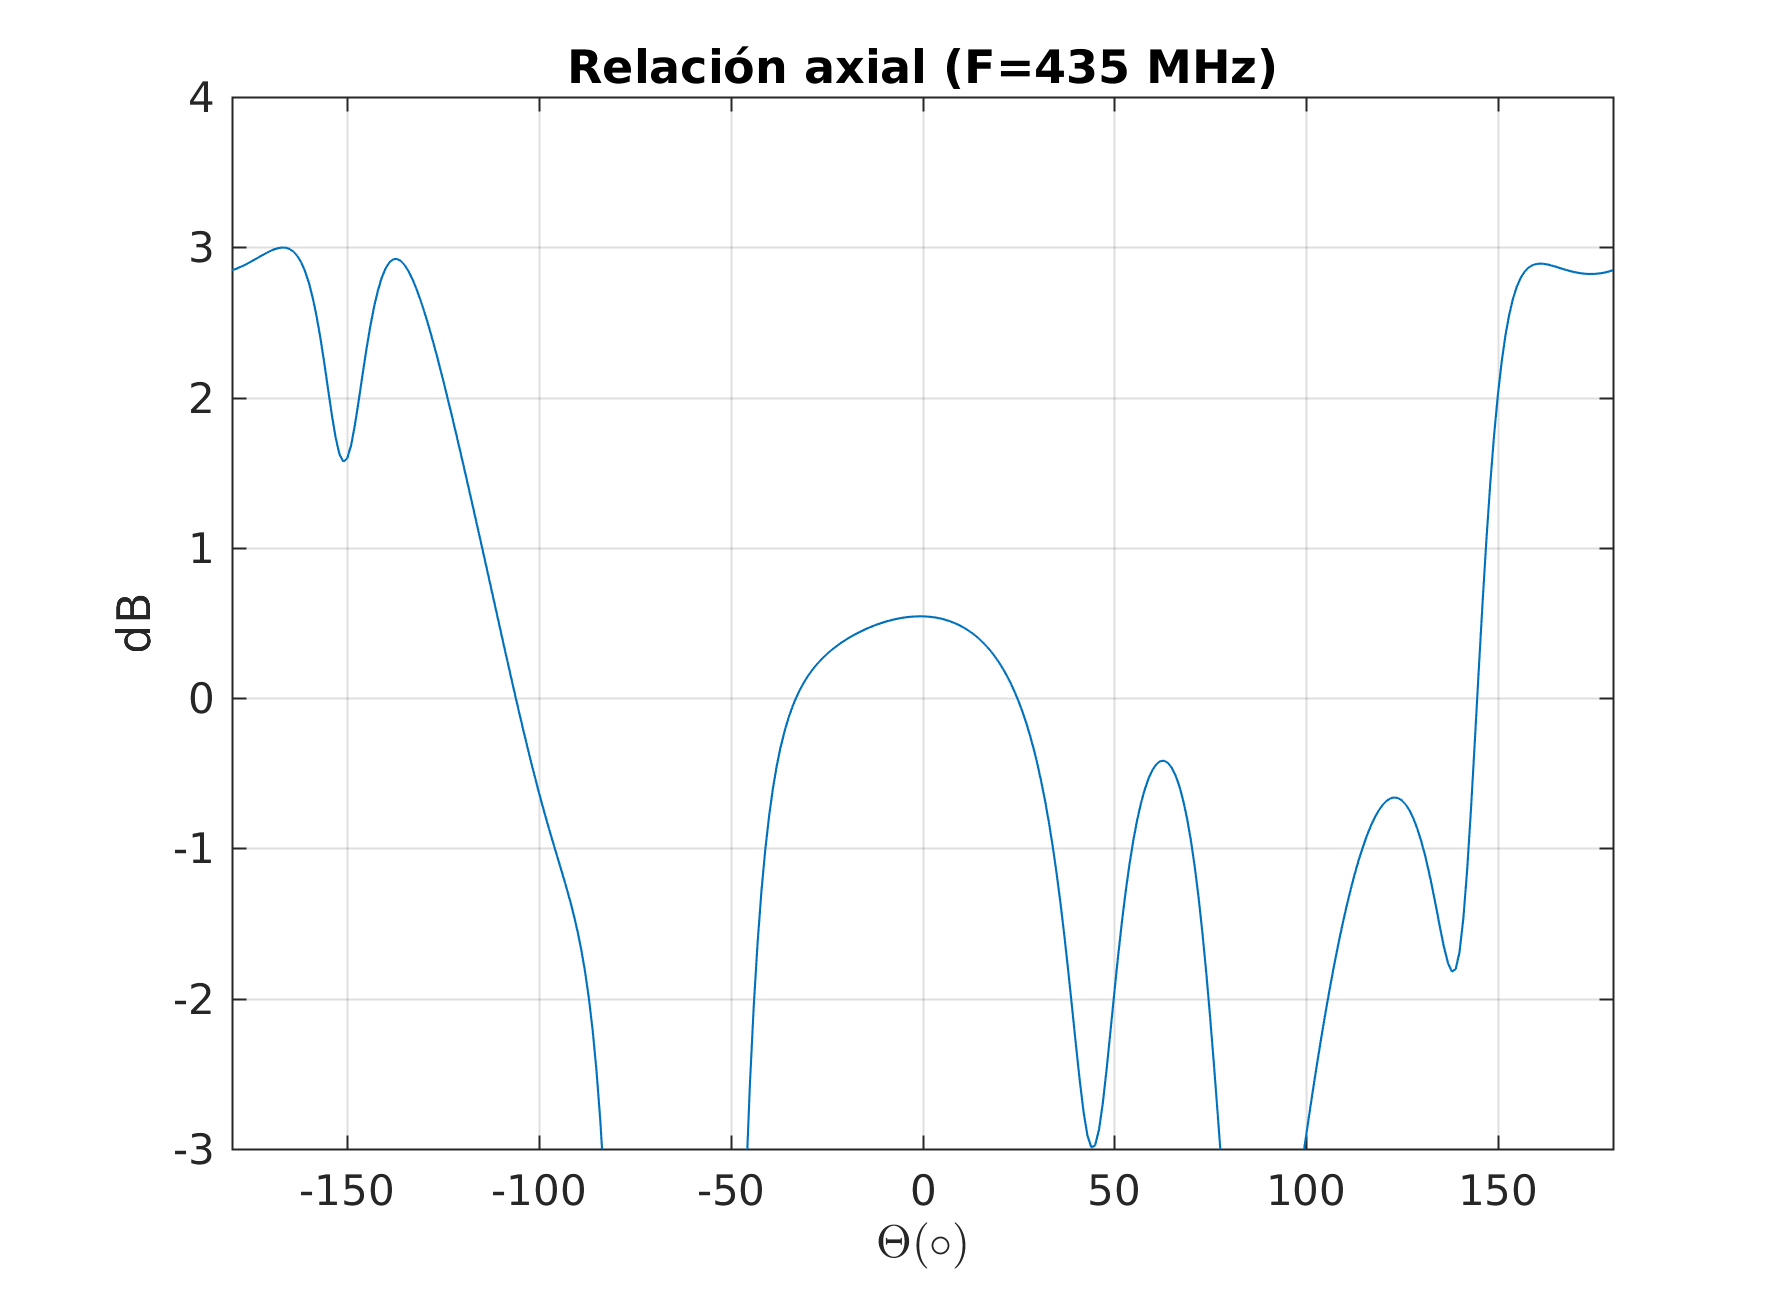
\includegraphics[width=0.6\textwidth]{helix_2_F435_AR.png}
	\caption{Relación axial}
\end{figure}


\end{document}
